\documentclass{article}
\usepackage[swedish]{babel}
\usepackage[utf8]{inputenc}
\usepackage[T1]{fontenc}

%Lägger till Referenser i Innehållsförteckningen
\usepackage{tocbibind}
\usepackage{float}
\usepackage{amsmath}
\usepackage{parskip}
\usepackage{todonotes}
\usepackage{url}
\usepackage{hyperref}
\usepackage{multicol}

\title{Larmsystem baserat på MD407-mikrodatorer}

\author{\large Grupp 13\\Filip Borg, Gustav Fåhraeus, Josef Karlsson,\\
Erik Nilsson, Adam Thörnblom, Ben Wooldridge}
\date{Läsperiod 1, HT-2019\\DAT290 Datatekniskt projekt\\Datateknik}

% I utvärderingen granskas hur väl studenterna i sina rapporter har lyckats visa att de genom de teknikutvärderingar, konstruktionsval, tester och analys som de har gjort har förstått de problem de har ställts inför, samt hur de på basis av denna förståelse och utifrån rådande förutsättningar har lyckats agera för att lösa dessa problem.

% Kriterierna är läsarorienterade vilket innebär att de ska bedöma en utomstående läsaresmöjligheter att förstå rapporten. Rapporten ska först och främst ses som ett dokument vars läsare finns inom organisationen där arbetet sker,men det ska kunna läsas och förstås av personer som inte har jobbat med och därför inte är insatta i projektet, exempelvis en nyanställd som inte känner till projektet och dess bakgrund, en anställd i en annan organisation med liknande verksamhet eller en ingenjörsstudent inom datateknik som har gått en liknande utbildning på en annanhögskola.

% En bakåtsyftande projektrapport: “Rapporten beskriver utvecklingen av…”




\begin{document}

%Titelsida
\maketitle
\pagenumbering{gobble}
\newpage

\tableofcontents
\newpage

\pagenumbering{arabic}

\section*{Beteckningar}
\begin{itemize}
    \item \textbf{MD407} – En ARM-baserad
    laborationsdator för utbildning
    \item \textbf{ARM} - En processor-arkitektur
    \item \textbf{CAN} - Controller Area Network
    \item \textbf{GPIO} - General-purpose input/output
    \item \textbf{USART} - Universal asynchronous receiver-transmitter
    \item \textbf{LED} - Light-emitting diode
\end{itemize}
\newpage

\section{Inledning}
Rapporten beskriver utvecklingen av ett modulärt larmsystem som i grunden består av ARM-baserade MD407-enkortsdatorer.


I en undersökning\cite{brott-foretagarna} utförd av Sveriges största företagsorganisaton, \textit{Företagarna}, anger var tredje företag (n=983) att de blivit utsatta för minst ett brott någon gång under de senaste fem åren. Pontus Lindström, ansvarig för brott- och trygghetsfrågor hos Företagarna säger:
\begin{quote}
\textit{- Undersökningen bekräftar den bild vi har. Många företagare vittnar om en ökad utsatthet och om att otryggheten ökat.}
\end{quote}

25\% av de företag som blivit utsatta för minst ett brott anger att de inte anmält brottet till polisen. 36\% anger att de anmält något brott de utsatts för, men inte alla. Den låga anmälningsgraden tyder på att företagen inte tycker att anmälningarna ger någonting.  Företagen anger att de känner sig tvungna att satsa stora summor på larmsystem, vilket finansiellt inte alltid är en lätt investering att göra, speciellt inte för små företagare utan kapital.

\subsection{Syfte} % Svarar på frågan "Varför"?
Larmsystemets syfte är att vara ett finansiellt dynamiskt alternativ för företag
och organisationer som har behov av anpassad larmning beroende på rådande behov.
Detta uppnås genom att erbjuda mindre delsystem som kan kopplas ihop till ett större centraliserat system.

Systemet ökar översikten och säkerheten av användarens lokaler genom att implementera konfigurerbar larmning av dörrar, samt rörelse- och vibrationsdetektering.

\subsection{Mål} % Svarar på frågan "Vad"?
% I detta avsnitt beskrivs koncist samtliga övergripande tekniska mål med projektet, det vill säga, vad som ska konstrueras. De mål som anges här kommer att styra projektets utveckling. När projektet närmar sig sitt slut och den slutliga projektrapporten lämnas in kommer beställaren att kritiskt analysera hur väl projektet lyckats genom att jämföra planens mål med den tekniska konstruktion som redovisas i projektrapporten.
Ett komplett larmsystem i minimal form består av 3 enheter:
\begin{itemize}
    \item 1st Dörrenhet
    \item 1st Rörelseenhet
    \item 1st Centralenhet
\end{itemize}
Samtliga enheter kräver en MD407-mikrodator för individuell drift. För att koppla samman
fristående enheter till ett centraliserat system krävs en CAN-buss.

Dörrenheten hanterar detektering och larmning av dörrar. Vid systemuppstart kontrollerar
dörrenheten antalet dörrar kopplade på enkortsdatorn. Datarepresentationer av dessa dörrar skapas, vilket möjliggör för dörrarna att efter en förutbestämd tid utlösa lokala larm genom att en LED-lampa på den larmande dörren tänds.
Dörrarna kan skicka centrala larm via en CAN-buss till centralenheten. Tider innan respektive larm utlöses kan konfigureras från centralenheten.
Från centralenheten kan dörrar också avlarmas, vilket hindrar samtliga larm på dörren från att utlösas.

Röreleseenheten består av en rörelse- och en vibrationssensor. Om endera sensor
utlöses skickas ett centralt larm via en CAN-buss till centralenheten. Känsligheten
på rörelsesensorn konfigueras från centralenheten. Vibrationssensorn konfigueras direkt på hårdvaran.

Centralenheten hanterar konfiguration av de andra enheterna, samt fungerar som en
central för samtliga larm som utlöses i systemet. Om ett centralt larm utlöses så
kan det endast ackkrediteras och nollställas via centralenheten.

\subsection{Arbetsmetod} % svarar på frågan "hur har vi gått tillväga i det tekniska utvecklingsarbetet"?
I det här avsnittet beskrivs det hur arbetet i gruppen delades upp, och hur gruppen har hanterat
filhantering, möten och arbetstid.
\subsubsection{Undergrupper}
För att jämna ut arbetsbelastningen delades projektgruppen in i tre grupper om två personer vardera,
en för varje enhetstyp.

\textbf{Centralenheten}: Gruppens uppgift var att kunna styra
periferienheterna från centralenheten samt implementera CAN och USART.

\textbf{Dörrenheten}: Dörrenheten ansvarar för att alla dörrar skall vara uppkopplade och larmade.

\textbf{Rörelseenheten}: Rörelseenheten utvecklar mjukvaran till
rörelse- och vibrationssensorerna för larmning av t.ex. fönster och värdefulla föremål.

\subsubsection{Möten och arbetstid}
Projektgruppen har haft ett möte varje vecka, där gruppen har gått igenom vad som gjorts
sedan det senaste mötet och även gått igenom vad som är nästa uppgift.

Projektgruppen har även haft två bestämda arbetstillfällen varje vecka. Utöver dessa bestämda arbetspass har gruppen jobbat i sina undergrupper. Under dessa tillfällen har undergrupperna även kunnat ta hjälp av andra undergrupper då gruppen har suttit i labbsalen.

Varje gruppmedlem har även lagt tid utanför dedikerad arbetstid.

\subsubsection{Fildelning och versionshantering}
Arbetsgruppen valde att använda versionshanteringstjänsten GIT för att förenkla den parallella programmeringen, och för att samla alla filer och dokument på ett ställe.


\section{Teknisk beskrivning} % Vad är utgångspunkten för i förkonstruktionsarbetet?
I det här avsnittet är det mer teknisk information om hur de olika delarna av
systemet fungerar, och om information som kan vara nödvändig för att förstå systemets
helhet. 
\subsection{Teknisk bakgrund}
Mjukvaran till larmsystemet körs på ett flertal MD407-kort, ett för varje enhet.
\subsection{Systemöversikt}

Systemet utgår från en centralenhet, kopplad till en dörrenhet och en rörelsenhet över en gemensam CAN-buss. Periferienheterna hanterar avmätning av sina respektive sensorer, samt begär larm via CAN-bussen vid behov. När det går ett centralt larm fortsätter larmet tills en användare slår av larmet via en pin-kod till centralenheten.

Dörrenheten är kopplad till ett antal strömbrytare/dörrsensorer, och larmar då en dörr är öppen för länge, först lokalt och sedan centralt.
Rörelseenheten är kopplad till ett antal avstånds- och vibrationsensorer, och larmar centralt om ett föremål detekteras av en avståndsmätare inom konfigurerbart avstånd.
Rörelseenheten larmar även centralt om en vibrationssensor mäter ett konfigurerbar antal vibrationer inom en viss tidsram. % Lite flummig beskrivning kanske, får ändra när koden är klar.

En översikt av hårdvaran och hur den är kopplad finns i Figur \ref{fig:hårdvara}.
\begin{figure}[H] % Samma figur som projektplanen, då hårdvaran fortfarande ser likadan ut, det är värt att göra en ny innan slutgiltiga rapporten.
    \centering
    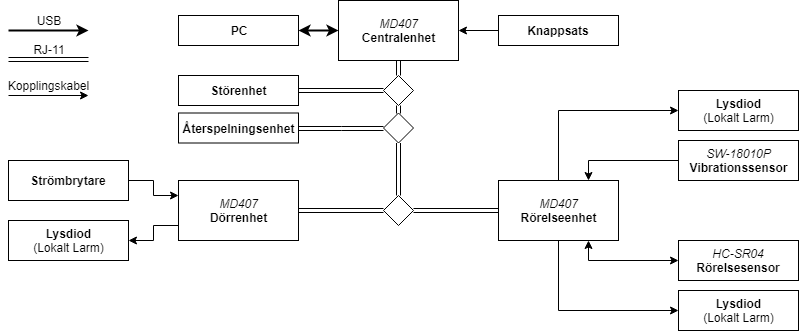
\includegraphics[width=1\textwidth]{figurer/HardvaraOversikt.png}
    \caption{Översikt över hårdvara}
    \label{fig:hårdvara}
\end{figure}

När centralenheten samt periferienheterna startar befinner de sig i konfigurationsläge,
 där varje enhet konfigurerar sig på lokal nivå (USART, CAN-bussen, GPIO), varpå centralenheten skickar konfigurationer till periferienheterna, som de använder för att konfigurera sina respektive sensorer.
 Efter att ha konfigurerats går enheterna in i var sin kontinuerlig loop. Periferienheterna mäter ständigt av sensorerna och skickar larm-meddelanden över CAN-bussen till centralenheten vid behov. Centralenheten skickar periodiskt konfigurationer till periferienheterna och larmar om dessa inte bekräftas.

En överblick av mjukvarans tidsflöde finns i Figur \ref{fig:tidsflöde}.

\begin{figure}[H]
    \centering
    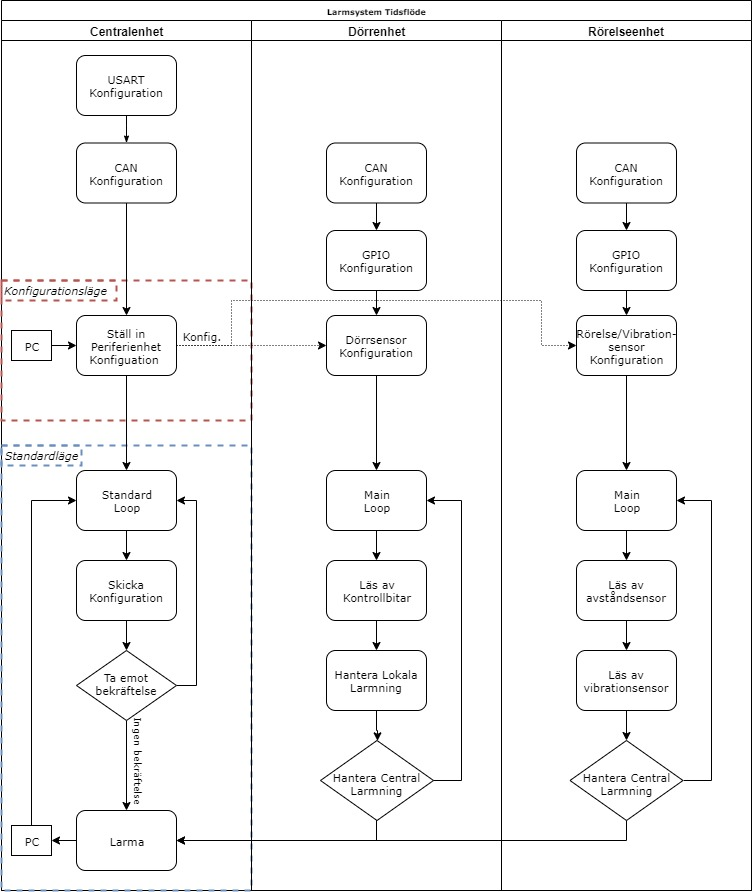
\includegraphics[width=1\textwidth]{figurer/TidsFlode.jpg}
    \caption{Tidsflöde Mjukvara}
    \label{fig:tidsflöde}
\end{figure}


\subsection{CAN-kommunikation}
\label{can}
\subsubsection{Beskrivning av CAN-protokollet}
Protokollet som har skapats för kommunikationen mellan enheterna bygger på protokollet Controller Area Network (CAN).
CAN är ett bussprotokoll som främst används för kommunikation mellan datorer och givare på fordon där det ställs höga krav på tillförlitlighet.
För att undvika kollisioner och därmed öka tillförlitligheten har CAN en dominant logisk nivå (0) som dessutom ger automatisk prioritering av meddelanden då den dominanta nivån har företräde på bussen.
Denna prioritering har använts för att ge brådskande meddelanden företräde över meddelanden som inte kräver kort responstid. I tabell \ref{tab:meddelandetyper} är de meddelandetyper som används kortfattat beskrivna. För en mer detaljerad beskrivning av protokollet och dess meddelandetyper, se bilaga \ref{bilaga:protokoll}.



\begin{table}[H]
	\centering
	\begin{tabular}{|c|p{0.65\textwidth}|}
		\hline
		Meddelandetyp & Används till \\ \hline \hline
		Bekräftelse		& Bekräftelse för senaste mottagna meddelandet. \\ \hline
		Skicka larm		& Talar om för centralenheten om någon dörr eller sensor larmar. \\ \hline
		Konfiguration		& Används för att skicka sensorkonfiguration och kalibrering. \\ \hline
		Tilldelning av ID		& Används då centralenheten tilldelar en periferienhet dess ID. \\ \hline
		ID-begäran		& Används för att begära ett ID. \\ \hline

	\end{tabular}
	\caption{Meddelandetyper som används för datakommunikationen.}
	\label{tab:meddelandetyper}
\end{table}


\subsubsection{Implementation}
För hantering av CAN-meddelanden har STM-biblioteket (se \ref{stm}) använts för inledande initiering,
hantering av avbrott och att skicka meddelanden.
Utöver det har ett system utvecklats för att hantera mottagna meddelanden med hjälp av avbrott.
Hanteringsfunktionen paras ihop med filtret för tillhörande meddelande.
Hanteringsfunktionen anropas sedan av avbrottsrutinen då ett meddelande passerat filtret.
Denna lösning har valts då de flesta meddelanden naturligt hanteras med en kort hanteringsfunktion
som inte kräver input från användaren.


\subsection{USART}
För att ge användaren möjlighet att interagera med systemet har Universal asynchronous receiver-transmitter (USART) implementerats. USART sköter kommunikationen mellan mikrodatorn och den terminal som används då mikrodatorn är ansluten till en dator. Via terminalen får användaren utskrifter från programmet och har även möjlighet att ge kommandon till systemet.


\subsection{Störenhet}
För att ge möjlighet att testa systemet på ett tungt trafikerat CAN-nätverk har en störenhet utvecklats. Störenheten skickar frekvent meddelanden med slumpartat innehåll. Hastigheten är reglerbar via USART. Utöver att generera brus kan enheten också fungera som en lyssnare med avaktiverad störfunktion.


\subsection{Delsystem }
\subsubsection{Centralenheten}
%\label{subsec:centralenhet}
Centralenheten styr och har uppsikt över övriga enheter.
Inställningar görs via USART med kommanodon enligt Appendix \ref{kommandon}, varpå de vidarebefordras till rätt periferienhet via CAN.

Centralenheten har följande två lägen:

\begin{enumerate}
    \item Standardläge: Enheten väntar på larm-meddelanden från periferienheterna eller användarinput via USART. Dessutom skickar den regelbundet konfigurationen för anslutna dörrar och sensorer till periferienheterna, som förväntas bekräfta konfigurationen.
    Om en enhet inte svarar efter ett visst antal meddelanden går larmet.
    \item Konfigurationsläge: Detta är det läge enheten startar i.
    Här kan användaren konfigurera anslutna dörr- och rörelseenheter via USART. Användaren kan sätta centralenheten i konfigurationsläge via USART för att lägga till eller konfigurera periferienheter.
\end{enumerate}

För att kunna adressera olika periferienheter måste centralenheten tilldela dessa varsitt unikt id.
Detta görs i konfigurationsläget genom att varje enhet som saknar id skickar en förfrågan via CAN.
När centralenheten tar emot en sådan förfrågan från en periferienhet, skickar den tillbaka det
lägsta lediga id:t och skapar en ny instans av en struktur som representerar periferienheten och lägger den i en lista. Strukturen innehåller enhetens id och konfiguration (d.v.s. tider för varje dörr för dörrenheter respektive avstånd för varje avståndssensor och antal vibrationssensorer för rörelseenheter).
Id:t används för att adressera meddelanden till samt identifiera meddelanden från enheten. Det är också
periferienhetens index i centralenhetens lista, vilket gör det oerhört effektivt att hitta rätt
enhet i listan när dess id har lästs i CAN-meddelandet.





\subsubsection{Dörrenheten}
\label{subsec:Dörrenheten}
% Punkter att få med:
% - Systemuppstart
% - Lokala / Centrala Larm
% - CAN
% - Initiering?
% - Systick?
% - Bilder?

Dörrenheten är en av systemets fristående enheter och kräver en MD407-mikrodator för drift.

För att koppla upp en dörr till systemet krävs det två anslutningar till en av mikrodatorns
 GPIO-portar: en koppling som går från en strömbrytare på dörren till en av mikrodatorns jämna
  I/O-pinnar (\textit{n}), samt en koppling från en LED-lampa på dörren till en ojämn I/O-pinne (\textit{n+1}).

Fyra av mikrodatorns fem portar är designerade för dörranslutningar (\textit{A,C,D,E}). \\
Eftersom samtliga portar har 16 tillgängliga pinnar innebär detta att systemet maximalt kan stötta 32 dörrar per dörrenhet.

Port B är inte avsedd för dörranslutningar, utan används främst för CAN-\\kommunikationen
med centralenheten. En LED-lampa kan även kopplas till \\ pinne 2 på port B. Denna lampa är
till för att vid uppstart signalera när systemets initiering är färdig.

Vid uppstart initieras först portarna och pinnarna på mikrodatorn så att de kan adresseras
och avläsas på rätt sätt. Därefter startas en System Timer (SysTick) som fungerar som klocka, och
Can som initieras som används för att enheten ska kunna kommunicera
med en eventuell centralenhet. För att kunna representera sig på Can-bussen initieras även
en 32 bitars slumptals generator som är enhetens id tills att den fått ett designerat av
centralenheten. Fortsättningsvis detekterar systemet hur många dörrar som är kopplade 
på kortet, och på vilka pinnar de är kopplade. För att dörrarna ska kunna detekteras krävs det att
 de är stängda.

Under detekteringen skapas datarepresentationer med förinställda värden för de dörrar som systemet
detekterar. Efter att samtliga datarepresentationer är skapade kommer systemet att försöka begära 
ett id av en eventuell centralenhet. Ifall systemet inte får ett id inom 20 sekunder kommer systemet 
gå in i lokal drift. Oavsett ifall systemet lyckats få ett id kommer den forsätta med att tända dörrarnas lampor
i den ordning de initierades. Detta görs för att testa om de lokala larmen fungerar hos dörrarna.
Efter att samtliga lampor är tända så släcker systemet dem igen.
Slutligen tänds lampan som är kopplad till pinne 2 på port B för att signalera till användaren att enheten är redo för drift.
Ifall systemet inte fått ett id kommer systemet kontinuerligt var 10 sekund skicka en
id begäran på can-bussen. Vilket gör att En dörrenhet kan startas och köras i lokaldrift
tills en centralenhet kopplas in i nätverket. När en centralenhet kopplas in på nätverket
kommer då systemet automatiskt att dyka upp hos centralenheten utan att användaren behöver
göra någonting på dörrenhetens sida.


\begin{figure}[H]
\begin{flushleft}
Systemet kontrollerar nu fortlöpande alla dörrar enligt flödesdiagrammet i figur 3: \linebreak \newline
\end{flushleft}
\centering
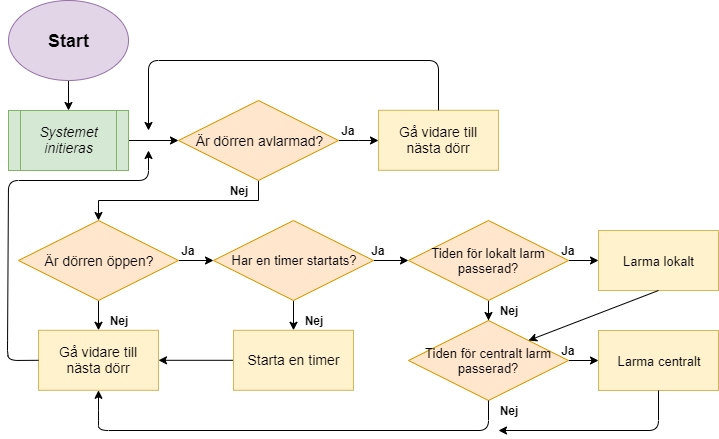
\includegraphics[scale=0.5]{figurer/Flow-Chart.png}
\caption{Flödesschema över dörrenhetens funktionalitet som visar vilka beslut systemet tar beroende på externa och interna händelser.}
\end{figure}

Dörrenhetens flöde bygger på polling. Samtliga dörrar har i sina datarepresentationer
ett antal kontrollbitar. I flödesschemat i figur 3 är dessa kontrollbitar representerade
som 'beslut' som anger huruvida en kontrollbit är satt till 1 (för \textit{ja}) eller 0
(för \textit{nej}). Dessa kontrollbitar sätts till 1 eller 0 beroende på externa händelser.

Avlarmning av en specifik dörr sker via CAN-kommunikation från centralenheten. Att en dörr är avlarmad
innebär att dess larm inte kan utlösas. Ifall ett larm redan har utlösts stängs det då också av.

Att en dörr är öppen innebär att kretsen som går via strömbrytaren på dörren inte längre är sluten.
Om kretsen inte är sluten, och dörren inte är avlarmad, tyder det på att någonting externt har hänt 
som systemet bör ta hänsyn till. Hur lång tid systemet väntar innan det larmar lokalt konfigureras i
 10-sekunders intervall via centralenheten. Väntetiden kan vara allt från 0 sekunder till ca 40 minuter
   (maxtiden är $2^8 *10$ sekunder).

När dörrenheten larmar centralt så skickas ett meddelande via CAN till centralenheten. Meddelanden
kommer skickas med intervall på en sekund tills centralenheten skickar tillbaka en ackreditering om att larmet har
 mottagits.

När dörrenheten larmar lokalt tänds en lampa för dörren, som kan kompleteras med ett tjutande ljud.
genom att koppla in en högtalare till AUX-porten. ifall användaren väljer att koppla in en högtalare
kommer dock enheten kunna stötta en dörr mindre. Detta är pågrund av att porten \textit{PA5} används
till högtalaren och kan då inte längre stötta en dörr.

Dörrenheten kan som tidigare nämnt köras utan uppkoppling till centralenheten. I det läget finns det dock inget centralt larm
och dörrar kan inte konfigureras utöver standard värdena som är förinställda.




\subsubsection{Rörelseenheten}
Denna periferienhet använder avståndsmätare av modellen HC-SR04 som rörelsesensorer, och vibrationssensorer av modellen SW-18010P, som styrs av en MD407-mikrodator.

Rörelseenheten använder mikrodatorns alla fem GPIO-portar, port A, B, C, D och E.
Port A, B och C används till rörelsesensorerna,
och port D och E till vibrationssensorerna.

Vid uppstart initieras först portarna och pinnarna på mikrodatorn så de kan adresseras och avläsas på rätt sätt. Därefter startas en System Timer (SysTick) som används som klocka.
Fortsättningsvis detekterar systemet hur många rörelse- och vibrationssensorer som är inkopplade till kortet, och på vilka pinnar de är kopplade. För att vibrationssensorerna skall detekteras får de ej utsättas för vibrationer under uppstart.

Efter detekteringen skapas datarepresentationer med förinställda värden för de sensorer som systemet hittat. Efter att samtliga datarepresentationer är skapade skickas en lista av de inkopplade sensorerna till centralenheten som bestämmer vilka sensorer som ska vara aktiva samt sätter larmavståndet för rörelsesensorerna.

Båda typerna av sensorer larmar och avlarmas endast via centralenheten, dock finns en LED-lampa lokalt
som blinkar till när ett larm går.

\textbf{Rörelsesensorn}:
En rörelsesensor tar upp tre pinnar. Varje port har därmed plats för fem sensorer.
Trig- och echo-pinnen från HC-SR04 samt en LED-lampan kopplas till  pin-n, -(n+1) respektive -(n+2).


Sensorn aktiveras genom att MD407-mikrodatorn skickar en hög puls till sensorn i minst 10 mikrosekunder, varpå sensorn skickar ut ultraljudsvågor och sänder en hög puls till MD407-mikrodatorn tills ultraljudsvågorna har återvänt. Avståndet till närmaste föremål beräknas genom att mäta längden på pulsen.
HC-SR04 kan mäta avstånd upp till 400 cm och larmavståndet är justerbart från centralenheten.

\textbf{Vibrationssensorn}: Sensorn sänder kontinuerligt en hög puls till MD407-mikrodatorn utom när den
känner av vibrationer, då den istället sänder en låg puls.
Sensorns känslighet justeras fysiskt genom en komparator på sensorn.



% Användarhandledning?

\section{Metoder}
\subsection{Tillvägagångsätt}
\label{tillvägagångsätt}
För att säkerhetställa det bästa möjliga resultatet för larmsystemet har det mesta arbetet bedrivits i samma
rum, vilket har låtit gruppen samråda om eventuella frågor eller funderningar från gruppmedlemmar.

\subsection{Verifikation}
\label{verifikation}
För att utvärdera huruvida larmsystemet uppnår de mål och krav som formulerats i målet används tester.
De tre undergrupperna har skrivit tester för sina respektive delsystem som försäkrar att
delsystemen fungerar enligt specifikationen. Ett test som är skrivet av en undergrupp utförs
av en annan undergrupp för att minimera partiskhet i utförandet.

Testet för det kompletta centraliserade systemet formulerades och utfördes av gruppen som helhet.

För att se samtliga testspecifikationer, samt resultat och analys, se bilaga \ref{bilaga:tester}.


\subsection{Programbibliotek}
\label{stm}
Programbiblioteket STM32\cite{stm} används för:
\begin{itemize}
    \item Initieringar av enkortsdatorernas GPIO.
    \item Implementation av en System Timer (SysTick).
    \item "Väntetid'-funktionalitet. (Delay-funktioner)
    \item Implementation av CAN-kommunikation.
\end{itemize}

STM används för att bespara projektgruppen jobb med att implementera \\ generell funktionalitet som redan skrivits för MD407-enkortsdatorer.

 \section{Resultat}
 För kompletta testspecifikationer hänvisas till bilaga \ref{bilaga:tester}.

 % Detta avsnitt redovisar resultatet av genomförd verifirering av systemet; dels fördelarna, dels för komplett system. Detta avsnitt redovisar även resultatet av det slutgiltiga fysiska testet när hela systemet körs i skarpt läge. Ni ska främst redovisa resultat i form av funktionalitet, men ta ocks upp prestanda aspekter om dessa är viktiga. Diskutea hur väl ni lyckats med er slutprodukt i förhållande till er projektplan.
 \subsection{Centralenheten}
 Centralenheten har följande funktionalitet:
 \begin{enumerate}
     \item Tilldelning av ID till periferienheter.
     \item Konfiguration av periferienheter via USART.
     \item Automatisk detektering av enheter som lämnar nätverket.
     \item Larmhantering.
 \end{enumerate}
 För att säkerställa att funktionalitet ovan fungerar utfördes följande tester:
 \begin{enumerate}
     \item Test av ID-tilldelning och larmmeddelnade se bilaga \ref{test:idLarm}.
     \todo{Kommer kompleteras med fler tester.}
 \end{enumerate}
 
 \subsection{Dörrenheten}
 Dörrenheten har följande funktionalitet:
 \begin{enumerate}
     \item Detektering av antalet stängda dörrar kopplade på enkortsdatorn.
     \item Signalering via LED-lampa som indikerar att dörrenhetens initiering är färdig.
     \item Lokal larmning via LED-lampa.
     \item Central larmning via CAN-buss.
     \item Går att konfiguera väntetider innan larm från centralenheten.
     \item Avlarmning av individuella dörrar från centralenheten.
     \item Lokal funktionalitet kräver inte uppkopplad centralenhet.

 \end{enumerate}
 För att säkerställa att funktionalitet ovan fungerar utfördes följande tester:
 \begin{enumerate}
     \item Test av pinnar för dörrar
     \item Test av lokal drift
     \item Test av ID-tilldelning och larm
 \end{enumerate}

 \subsection{Rörelseenheten}
 Rörelseenheten har följande funktionalitet:
 \begin{enumerate}
 	\item Automatiskt detektera antalet inkopplade rörelse- och vibrationssensorer vid uppstart.
	\item Larma vid upptäckt av vibrationer eller rörelse.
    \item Central larmning via CAN-buss.
	\item LED-lampa som signalerar när ett larm skickas till centralenheten.
	\item Konfigurerbart larmavstånd på rörelsesensorerna.
	\item Avlarmning via centralenheten
 \end{enumerate}
 För att säkerställa att funktionalitet ovan fungerar utfördes följande tester:
 \begin{enumerate}
     \item
 \end{enumerate}
 
 \subsection{Larmsystemet som helhet}
\section{Slutsats och diskussion}
% Detta avsnitt innehåller en sammanfattning av konstruktionen och en diskussion av resultatet. Om detta är möjligt, dra slutsatser av ert projekt och identifiera förbättringsmöjligheter. (Vilka kan vara användbara för en beställare)
Utifrån testresultaten kan slutsatsen dras att dörrenheten fungerar som den ska enligt målet.

\todo[inline]{inte färdig}

% Referenser enligtIEEE.
%För referenser
\bibliographystyle{IEEEtran}
\bibliography{referenser}

% Avslutningsvis så vill vi påminna om att projektets slutrapport, precis som projektplanen, ska vara projektintern, det väl säga att den ska beskriva det tekniska utvecklingsarbetet och bortse från att projektarbetet faktiskt organiserats inom ramen för en kurs.

\appendix
    \section{Utförlig beskrivning av meddelandetyper kommunikationsprotokoll}
    \label{bilaga:protokoll}
        \section*{Grundidé}
\label{sec:grundide}

Centralenheten sparar all status och datainformation, denna information kopieras regelbundet till perferienheterna via konfigureringsmeddelanden. Centralenheten har 2 lägen.

\begin{enumerate}
	\item Standard running. Här lyssnar man på larm från periferienheterna. Dessutom skickar man regelbundet  konfigurationen för anslutna dörrar och sensorer. Periferienheten svarar ok, om den inte svarar efter ett antal meddelande larmar man.
	\item Vid uppstart är centralenheten i konfigurationsläge. Nu kan man via USART konfigurera anslutna dörrlarmsenheter samt lörelselarm.
\end{enumerate}

Varje perferienhet förväntas ha en unik fysisk adress som kommer användas vid tilldelning av ID adresser. Likt fysiska MAC adresser och logiska IP adresser i ethernet.

\section*{Bitfördelning i identifieringsdelen av meddelandet}
\label{sec:bitfördelning}

Totalt 11 bitar (Utan att utöka med 18 bitar till)
\begin{description}
	\item{0-2:} Första bitarna är meddelandetyp. 3 bitar dvs 8 meddelandetyper.
	\item{3:} en bit för riktning. Från/till centralenheten. Kan ses som en 4e bit i meddelandetypen.
	\item{4-10:} 7 bitar:
		Om riktning är till centralenheten är bitarna sändarens ID.
		Om riktningen är från centralenheten beskriver bitarna mottagarens ID.
		Innan enheten har en egen ID används bara ettor.
\end{description}


\section*{Meddelandetyper lista}
\label{sec:meddelandetyper}

\begin{table}[H]
	\begin{tabular}{|c|l|p{2.6cm}|p{6cm}|}
		\hline
		N& Riktning & Meddelandenamn & Beskrivning \\ \hline \hline
		0 & p -> c & Ack & Acknowledgement för senaste meddelandet. \\ \hline
		1 & p -> c & Skicka larm & Talar för centralenheten om någon dörr eller sensor larmar. \\ \hline
		3 & Båda & Skicka konfiguration & Skickar konfiguration till periferienheten kontinuerligt. Fungerar även som ping. Perferienheterna skickar sina konfigurationener i andra riktingen vid uppstart. Rörelselarmet har mätvärden i denna typ av meddelande. \\ \hline
		4 & c -> p & Tilldelning av ID & Centralenheten tilldelar en periferienhet dess ID. Enheten identifieras med dess fysiska adress i meddelandet. Detta meddelande skickas bara då centralenheten är i konfigurationsläge (läge  2). \\ \hline
		5 & p -> c & Ny enhet här & Centralenheten tilldelar en periferienhet dess ID. Enheten identifieras med dess fysiska adress i meddelandet. Detta meddelande skickas bara då centralenheten är i konfigurationsläge (läge  2). \\ \hline
	\end{tabular}
	\label{tab:meddelandetyper}
\end{table}

\section*{Detaljinformation angående meddelandetyperna}
\label{sec:detaljinfo}
\textbf{Skicka konfiguration} \\
I datadelen av meddelande för dörrlarm borde det finnas:
\begin{itemize}
	\item Ett par bitar för addressen till dörren i fråga.
	\item En aktiveringsbit per dörr.
	\item En bit per dörr för avaktivering av pågående larm.
	\item Ett par bitar för varje tidsfördröjning.
\end{itemize}

I datadelen av meddelande för rörelsesensorlarm borde det finnas:
\begin{itemize}
	\item En aktiveringsbit per sensor
	\item En bit per sensor för avaktivering av pågående larm.
	\item En bit per enhet för aktivering av automatisk översändning av “Skicka larm och mätvärden” meddelanden. Detta kommer användas vid konfiguration av avståndsgivare.
\end{itemize}

\section*{Todo}
\label{sec:todo}
Borde man ha olika meddelandetyper för “Skicka larm” beroende på vilken enhetstyp det rör sig om?


    \section{Kommandolista för centralenheten}
    \label{kommandon}
        För att styra centralenheten används ett antal kommandon som beskrivs nedan. Då centralenheten har två separata lägen.

    
    \textbf{help}\\
    Används för att se de tillgängliga kommandona för det aktiva läget (standard eller konfiguration).

    \textbf{start}\\
    Startar standardläge.

    \textbf{dor v x y z}\\
    Där \textbf{v, x, y} och \textbf{z} är tal mellan 0 och 9. Konfigurerar dörr \textbf{x} på enhet med ID \textbf{v} med timer för lokalt larm på  \(\textbf{y} * 10\) sekunder samt en fördröjning till centralt larm på \(\textbf{z} * 10\) sekunder.

    \textbf{ror x y z}\\
    Där \textbf{x, y} och \textbf{z} är tal mellan 0 och 9. Konfigurerar rörelsesensor \textbf{y} på enhet med ID \textbf{x} för att larma då den detekterar ett föremål på ett avstånd mindre än \(\textbf{z} * 10\) centimeter.

    \textbf{avlarma y z} \\
    Avlarmar sensor \textbf{z} på enhet med ID \textbf{y}.

    \textbf{larma y z} \\
    Larmar sensor \textbf{z} på enhet med ID \textbf{y}. Alla sensorer är larmade som standard så detta kommando körs om man vill återaktivera larm efter att det avaktiverats.

	\clearpage
	\section{Tester}
    		\label{bilaga:tester}
     	%Beskrivande titel av testet samt en unik label
\subsection{Test av pinnar för dörrar}
\label{test:portTest}

\setlength{\columnsep}{1cm}


% Vid utförande av test fylls mallen nedan i, vilket resulterar i ett protokoll som sedan sparas som verifikation. Målet med dessa protokoll är att man utan sakkunskap ska kunna skapa sig en överblick av att systemet fungerar som det ska.


\begin{multicols}{2}
\subsubsection*{Test formulerat av}
% Namn på den/de som formulerade testet.
Adam

\subsubsection*{Utfört av}
% Namn på den/de som utförande testet.
Filip


\end{multicols}
\subsubsection*{Komponent}
%Vilken del av systemet testas?
Dörrenheten


\subsubsection*{Testsyfte}
%Vad ska testet visa? Är testet till följd av tidigare test?
Säkerställa att alla portar fungerar.


\subsubsection*{Hjälpmedel}
%Lista hjälpmedlen som användes i samband med testet.
\begin{itemize}
	\item Ledlampor
	\item Dörrbrytare
	\item Kopplingskapel
	\item kopplingsbräda
\end{itemize}



\subsubsection*{Utförande}
%Hur ska testet utföras?
Testa portarna A, C, D och E  en åt gången genom att koppla in dörrbrytare på pinnar med jämt index (0,2,4..) och tillhörande ledlampor på pinnarna ovanför (1,3,5..). Kör sedan programkoden för dörrenheten och vänta tills initsieringen är utförd och programet är i lokal drift. Ta nu bort magneten från dörrbrytaren och kontrollera så att tillhörande lampa tänds.


\subsubsection*{Resultat}
%Vad är testresultatet? Hittades några buggar?
Lamporna tänds som dem ska.



\subsubsection*{Analys}
%Vad innebär testets resultat? Behövs fler test av komponenten? Behöver andra komponenter testas ytterligare, och i så fall hur?
De använda portarna fungerar som dem ska.



         \clearpage
%Beskrivande titel av testet samt en unik label
\subsection{Test av ID-tilldelning och larm}
\label{test:idLarm}

\setlength{\columnsep}{1cm}


% Vid utförande av test fylls mallen nedan i, vilket resulterar i ett protokoll som sedan sparas som verifikation. Målet med dessa protokoll är att man utan sakkunskap ska kunna skapa sig en överblick av att systemet fungerar som det ska.


\begin{multicols}{2}
\subsubsection*{Test formulerat av}
% Namn på den/de som formulerade testet.
Adam och Filip

\subsubsection*{Utfört av}
% Namn på den/de som utförande testet.
Erik


\end{multicols}
\subsubsection*{Komponent}
%Vilken del av systemet testas?
Centralenhet och dörrenhet



\subsubsection*{Testsyfte}
%Vad ska testet visa? Är testet till följd av tidigare test?
Kontrollera att dörrenheten blir tilldelad ett ID av centralenheten vid uppstart. Därefter ska dörrenheten larma om dörrbrytaren bryts.


\subsubsection*{Hjälpmedel}
%Lista hjälpmedlen som användes i samband med testet.
\begin{itemize}
	\item CAN-kabel
	\item Dörrbrytare
	\item kopplingskabel
	\item CAN-lyssnare
\end{itemize}



\subsubsection*{Utförande}
%Hur ska testet utföras?
Koppla upp en dörrbrytare på en port (A, C, D eller E). Därefter kopplas CAN-nätverket upp med lyssnare, centralenhet och dörrenhet. Starta sedan lyssnaren och centralenheten. Se till att centralenheten är i konfigurationsläge och starta därefter dörrenheten. Kontrollera nu att ID-tilldelningen sker genom att kolla på kommunikationen som lyssnare detekterar samt utskriften från centralenheten. 

Efter ID-tilldelningen är färdig sätts centralenheten i standarsläge genom att skriva kommandot start i konsolen. Testa nu att centralenheten detekterar larm som skickas från dörrenheten då dörrbrytaren öppnas. Läs första byten av meddelandet, här skickas ID till dörrenheten och ska vid detta läge vara 0.

Starta om dörrenheten och utför samma test igen. Denna gång ska IDt vara 1.


\subsubsection*{Resultat}
%Vad är testresultatet? Hittades några buggar?
ID-tilldelningen sker som den ska. Larmet skickas efter ett par sekunder efter att dörrbrytaren öppnats och mottas av centralenheten med en utskrift i konsolen.


\subsubsection*{Analys}
%Vad innebär testets resultat? Behövs fler test av komponenten? Behöver andra komponenter testas ytterligare, och i så fall hur?
ID-tilldelningen utförs korrekt och dörrenheten kan därefter larma om en öppen dörrbrytare detekterats.



         \clearpage
%Beskrivande titel av testet samt en unik label
\subsection{Test av lokal drift för dörrenhet}
\label{test:localDrift}

\setlength{\columnsep}{1cm}


% Vid utförande av test fylls mallen nedan i, vilket resulterar i ett protokoll som sedan sparas som verifikation. Målet med dessa protokoll är att man utan sakkunskap ska kunna skapa sig en överblick av att systemet fungerar som det ska.


\begin{multicols}{2}
\subsubsection*{Test formulerat av}
% Namn på den/de som formulerade testet.
Adam

\subsubsection*{Utfört av}
% Namn på den/de som utförande testet.
Erik


\end{multicols}
\subsubsection*{Komponent}
%Vilken del av systemet testas?
Dörrenheten


\subsubsection*{Testsyfte}
%Vad ska testet visa? Är testet till följd av tidigare test?
För att säkerställa att dörrenheten körs lokalt ifall ingen central enhet hittas.


\subsubsection*{Hjälpmedel}
%Lista hjälpmedlen som användes i samband med testet.
\begin{itemize}
	\item Ledlampor
	\item Dörrbrytare
	\item Kopplingskapel
	\item kopplingsbräda
\end{itemize}



\subsubsection*{Utförande}
%Hur ska testet utföras?
Starta upp dörrenheten utan att den är kopplad till en centralenhet.
Kontrollera så att efter ca 60 sekunder tänds statuslampan
på dörrenheten. Kolla även att dörrenhetens funktionalitet 
fungerar som den ska. 


\subsubsection*{Resultat}
%Vad är testresultatet? Hittades några buggar?
Lamporna tänds som det ska.



\subsubsection*{Analys}
%Vad innebär testets resultat? Behövs fler test av komponenten? Behöver andra komponenter testas ytterligare, och i så fall hur?
Det fungerar som det ska.



         \clearpage
%Beskrivande titel av testet samt en unik label
\subsection{Test av systemet med brus}
\label{test:brusTest}

\setlength{\columnsep}{1cm}


% Vid utförande av test fylls mallen nedan i, vilket resulterar i ett protokoll som sedan sparas som verifikation. Målet med dessa protokoll är att man utan sakkunskap ska kunna skapa sig en överblick av att systemet fungerar som det ska.


\begin{multicols}{2}
\subsubsection*{Test formulerat av}
% Namn på den/de som formulerade testet.
Filip

\subsubsection*{Utfört av}
% Namn på den/de som utförande testet.
Adam och Erik


\end{multicols}
\subsubsection*{Komponent}
%Vilken del av systemet testas?
Hela systemet dvs centralenhet, rörelseenhet och dörrenhet.


\subsubsection*{Testsyfte}
%Vad ska testet visa? Är testet till följd av tidigare test?
Kontrollera att systemet fungerar även om CAN-bussen är tungt belastad av brus.


\subsubsection*{Hjälpmedel}
%Lista hjälpmedlen som användes i samband med testet.
\begin{itemize}
	\item Centralenhet
	\item Rörelseenhet
	\item Dörrenhet
	\item Brusenhet
\end{itemize}



\subsubsection*{Utförande}
%Hur ska testet utföras?
Testet utförs först med rörelseenheten och dörrenheten inviduellt därefter testas båda enheterna samtidigt.

Koppla upp centralenhet, periferienheten med minst en aktiv sensor och brusenheten på ett CAN-nätverk. Starta brusenheten och dess brusgenerering med en hög fördröjning på 64 millisekunder. Starta nu periferienheten samt centralenheten och starta systemet som det vanligtvis görs. Efter initiering kontrolleras så att larm fungerar. Fungerar detta kan intensiteten på bruset ökas genom att minska fördröjningen. Upprepa därefter samma procedur som tidigare tills det slutar att fungera eller om maximal intensitet uppnåtts.


\subsubsection*{Resultat}
%Vad är testresultatet? Hittades några buggar?
Dörrenheten: Idbegäran och larm fungerade som de skulle under påverkan av mycket brus. Det var ingen skillnad mellan de olika nivåerna av brus.

Rörelseenhet: För att spara tid började vi direkt med maximalt brus dvs 1ms mellan meddelandena. Då detta fungerade som tänkt avslutades testet.


\subsubsection*{Analys}
%Vad innebär testets resultat? Behövs fler test av komponenten? Behöver andra komponenter testas ytterligare, och i så fall hur?
Enheterna klarar av att begära ID och larma trots att bussen är fylld med brus.


         \clearpage
%Beskrivande titel av testet samt en unik label
\subsection{Test av återspelningsenheten}
\label{test:replayer}

\setlength{\columnsep}{1cm}


% Vid utförande av test fylls mallen nedan i, vilket resulterar i ett protokoll som sedan sparas som verifikation. Målet med dessa protokoll är att man utan sakkunskap ska kunna skapa sig en överblick av att systemet fungerar som det ska.


\begin{multicols}{2}
\subsubsection*{Test formulerat av}
% Namn på den/de som formulerade testet.
Filip

\subsubsection*{Utfört av}
% Namn på den/de som utförande testet.
Gustav


\end{multicols}
\subsubsection*{Komponent}
%Vilken del av systemet testas?
Återspelningsenheten


\subsubsection*{Testsyfte}
%Vad ska testet visa? Är testet till följd av tidigare test?
Säkerställa att återspelaren klarar av att spela in och återge en kort kommunikationssekvens.
Testet avser både fördröjningar mellan meddelanden och meddelandenas korrekthet.


\subsubsection*{Hjälpmedel}
%Lista hjälpmedlen som användes i samband med testet.
\begin{itemize}
	\item Återspelare
	\item Brusenhet
\end{itemize}



\subsubsection*{Utförande}
%Hur ska testet utföras?
Koppla ihop återspelaren med brusenheten på CAN-bussen och starta sedan båda enheterna.
Se till att brusenheten ger utskrift för skickade meddelanden, se kommandolistan vid uppstart för att hitta rätt kommando.
Starta nu inspelning på återspelningsenheten, konsultera åter igen kommandolistan.
Nu ska en sekvens av meddelanden skickas på ett kontrollerat sätt på bussen.
Använd funktionen för att skicka ett slumpartat meddelande från brusenheten.
Skicka förslagsvis en kaskad av  ca 5 meddelanden följt av ett längre uppehåll på runt 10 sekunder, skicka slutligen ett par avslutande meddelanden.
Därefter avslutas inspelningen på återspelaren.

Kontrollera nu att brusenheten ger utskrift för mottagna meddelanden och starta därefter återspelningen på återspelningsenheten med cyklisk uppspelning.
Låt meddelandesekvensen återspelas två gånger.
Lägg ingen större vikt vid att kontrollera meddelandenas innheåll det kan göras efteråt, däremot borde fokus läggas på fördröjningarna.
Avlsuta återspelningen och kontrollera meddelandenas korrekthet genom att bräddra tillbaka genom historiken.


\subsubsection*{Resultat}
%Vad är testresultatet? Hittades några buggar?
Resultatet blev att återuppspelningsenheten spelade upp meddelandena i samma ordning, med samma tempo, och med samma innehåll som skickades initialt.



\subsubsection*{Analys}
%Vad innebär testets resultat? Behövs fler test av komponenten? Behöver andra komponenter testas ytterligare, och i så fall hur?
Testets resultat innebär att återuppspelningsenheten fungerar korrekt. I mån av tid kan kommandolistan på återspelningsenheten göras mer lättläslig.



         \clearpage
%Beskrivande titel av testet samt en unik label
\subsection{Återuppspelningsattack test}
\label{test:sessionID}

\setlength{\columnsep}{1cm}


% Vid utförande av test fylls mallen nedan i, vilket resulterar i ett protokoll som sedan sparas som verifikation. Målet med dessa protokoll är att man utan sakkunskap ska kunna skapa sig en överblick av att systemet fungerar som det ska.


\begin{multicols}{2}
\subsubsection*{Test formulerat av}
% Namn på den/de som formulerade testet.
Filip

\subsubsection*{Utfört av}
% Namn på den/de som utförande testet.



\end{multicols}
\subsubsection*{Komponent}
%Vilken del av systemet testas?
Alla tre enheter.


\subsubsection*{Testsyfte}
%Vad ska testet visa? Är testet till följd av tidigare test?
Kontrollera att session ID fungerar som skydd mot en återuppspelningsattack.


\subsubsection*{Hjälpmedel}
%Lista hjälpmedlen som användes i samband med testet.
\begin{itemize}
	\item Centralenhet
	\item Rörelseenhet
	\item Dörrenhet
	\item Återuppspelare
\end{itemize}



\subsubsection*{Utförande}
%Hur ska testet utföras?
\todo[inline]{Förtydliga hur man accepterar standardkonfiguratioen från periferienheten.}
Utför detta test först för dörrenheten sedan för rörelseenheten.


Se till att SESSIONIDACTIVE är definerat som 0 i startup.c för centralenheten.
Om inte ändra så att den är och kompilera om.
Koppla upp ett CAN-nätverk med centralenhet, periferienhet samt återspelare.
Starta inspelning på återspelaren och starta därefter de andra enheterna.
Initiera standardkonfigurationen för enheten och övergå till standadläge på centralenheten genom att köra kommandot start.
Låt nu systemet köra i några minuter (typ 3-5) utan att något larm går.
Skulle något larm gå startas testet för periferienheten om.
Avsluta inspelningen på återspelaren men frånkoppla inte matningen, då försvinner de inspelade meddelandesekvensen.


Stäng av de övriga enheterna och låt nu endast centralenheten och återspelaren vara inkopplade på nätverket.
Starta återuppspelning av den inspelade sekvensen.
Starta seden centralenheten och kontrollera att en periferienhet ansluter trots att den saknas på nätverket.
Godkänn standardkonfigurationen och övergå sedan till standardläge på centralenheten.
Om centralenheten nu tror att den kommunicerar med en periferienhet utan att larma har en återuppspelningsattack utförts.
Stäng av alla enhter.

Återupprepa nu testet med SESSIONIDACTIVE definerat till 1, dvs sessionID funktionen aktiverad.

Utför slutligen hela testet med en rörelseenhet i stället för en dörrenhet.



\subsubsection*{Resultat}
%Vad är testresultatet? Hittades några buggar?
Rörelseenheten: Med session-ID avaktiverat lyckades återuppspelningsattacken. Med session-ID aktiverat så kunde återuppspelaren ansluta som rörelseenhet, men när centralenheten startade larmade det. 


\subsubsection*{Analys}
%Vad innebär testets resultat? Behövs fler test av komponenten? Behöver andra komponenter testas ytterligare, och i så fall hur?




\end{document}
